\documentclass[letterpaper]{article}
\usepackage{iccc}

\usepackage{times}
\usepackage{helvet}
\usepackage{courier}
\usepackage{xcolor}
\usepackage{graphicx}
\usepackage{url}
\usepackage{fancyvrb}
\usepackage{paralist}

% ====================== CUSTOM COMMANDS 
%\DeclareMathAlphabet\mathbfcal{OMS}{cmsy}{b}{n}
\newcommand{\dref}[1]{Definition~\ref{#1}}
\newcommand{\eref}[1]{Equation~\ref{#1}}
\newcommand{\fref}[1]{Figure~\ref{#1}}
\newcommand{\tref}[1]{Table~\ref{#1}}
\newcommand{\sref}[1]{Section~\ref{#1}}
\newcommand{\aref}[1]{Algorithm~\ref{#1}}
\newcommand{\lpipe}{\rule[-0.4ex]{0.41pt}{2.3ex}\xspace}
\newcommand{\citeA}[1] {\citeauthor{#1}~(\citeyear{#1})}
\newcommand{\citeeg}[1] {(e.g. \citeauthor{#1}~\citeyear{#1})}

% Notes for draft-editing. I suggest you put your initials in the 
% first text env., and the note in the second text env.
% Syntax: \note
\def\note#1#2{\noindent {\color{red} {[\bf{#1}: {\it #2}]}}}

% ====================== DOCUMENT STYLING
\hyphenpenalty=5000


% ====================== DOCUMENT METADATA
\pdfinfo{
	/Title (Discourse-driven Comic Generation)
	/Subject (Proceedings of ICCC)
        /Author (Anonymous)
% XXX unblind:
% /Author (Chris Martens, Rogelio E. Cardona-Rivera)
}
%
\title{
        Discourse-driven Comic Generation
        \break
        {\small
	(Paper type: System Description)}
%	Toward Computational Comic Generation: \break
%	Exploring a Discourse-first Approach to Visual Narrative \break
%	Paper type: System Description
}
% XXX add this back for unblind
\author{
  Anonymous for review
}
% \author{
% 	Chris Martens\\
% 	Expressive Intelligence Studio\\
% 	Computational Media Department\\
% 	University of California, Santa Cruz\\
% 	Santa Cruz, CA, USA\\
% 	crmarten@ucsc.edu\\
% 	\And
% 	Rogelio E. Cardona-Rivera\\
% 	Liquid Narrative Group\\
% 	Department of Computer Science\\
% 	North Carolina State University\\
% 	Raleigh, NC, USA\\
% 	recardon@ncsu.edu\\
% }
\setcounter{secnumdepth}{0}

\begin{document} 
\maketitle
\begin{abstract}
	\begin{quote}
	Comics use sequences of still, two-dimensional visual stimuli to tell
stories, and they are deeply entwined with humanity's creative history.
While there is prior work on computationally generating discourse
(conveyance of narrative) for textual stories, few attempts have been made
to target comics, which carry distinct challenges and affordances, as a
discourse language.  Standard pipeline-based approaches to narrative
generation, wherein a discourse is configured only after a fabula has been
fixed, do not map well onto the affordances of purely visual panel
sequences.

% XXX can we back up this claim more strongly?

% Prior efforts toward comic-authoring computer programs mainly
% conform to fixed panel contents which cannot be flexibly rearranged
% while retaining narrative coherence.

% solution we propose
We propose a {\em discourse-first} scheme for generating comics, including novel configurations
of panel contents, by combining a
bottom-up panel sequencer inspired by McCloud's taxonomy of panel
transitions and a top-down grammar of comic arcs devised by Cohn.
% results
Our approach yields a flexible algorithm for comic generation whose output
can be rendered with a number of visual palettes, for which we have built
one proof-of-concept example and observed a wide range of variability in
output. Our efforts represent a first step toward robust comic generation
and provide a platform for analyzing and evaluating the validity of visual
discourse theories.



	\end{quote}
\end{abstract}


%% Paper:
%================================================================
\section{Introduction}

% XXX - maybe update this intro for ICIDS.
The computational generation of stories (hereafter {\em narrative
generation}) can help us understand some of the most creative aspects of
human intelligence~\cite{boyd2009origin}, such as reasoning about possible
and impossible worlds, and weaving narratives around our daily
lives~\cite{herman2013storytelling}.  Historically, narrative generation
has followed what Ronfard and Szilas \cite{ronfard2014story} term the
\emph{pipeline model}: a narrative artifact is generated by
first simulating the story world to form a collection of events, and then piping
the event information to a discourse generator, which generates a
selective presentation of story world events in a particular medium. A great
deal of existing work in narrative generation has primarily pursued this
pipeline model~\cite{gervas2009computational}. 
% XXX - update citation for ICIDS?

However, as Ronfard and Szilas argue, the pipeline model is neither
necessary nor sufficient for narrative generation.  Human authors
intentionally design their narratives to affect audiences in specific ways,
which involves reasoning about how story events are communicated more than
which story events occur~\cite{chatman1980story,bordwell1989making}. It is
unnecessary to simulate an aspect of the narrative universe that is never
communicated to the audience, if it does not inform the ultimate delivery
of the narrative artifact. It is also insufficient to reason about story
independent from discourse and medium, as the characteristics of a
discourse realization constrain the stories that can be told in that
medium~\cite{herman2004toward}.  The pipeline model unnecessarily restricts
how creative the generator can ultimately be, since story world commitments
are not revisited when generating discourse. Further, as will be detailed
later, narrative authorship depends on audiences being able to fill in the
gaps left open in the consumption of a
story~\cite{saraceni2016relatedness,magliano2016filling}.

Most prior work that uses the pipeline model implicitly assumes text, or
spoken verbal language, as the output generation medium, which allows the
pipeline model to avoid some of its limitations by baking medium
assumptions into the story model. For example, narrative generators can
model updates to internal character state, such as emotion or knowledge
change, which can simply be described in text. Communicating those
occurrences visually poses a significantly greater challenge.
Thus, we propose a simple kind of {\em visual} narrative as a testbed for
discourse generation: wordless comics, as in Figure~\ref{fig:calvin}. 
Comics are a relatively unexplored
domain of computational narratology~\cite{mani2012computational}, and they
present a wide range of expressive opportunities not afforded by text.

\begin{figure}
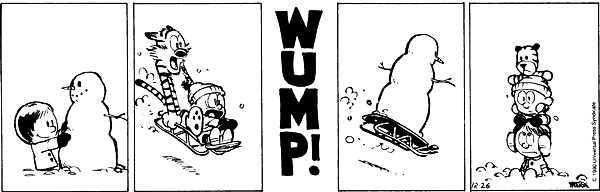
\includegraphics[width=\columnwidth]{calvin-and-hobbes.png}
\caption{
This wordless Calvin and Hobbes comic strip ({\small \copyright}~Bill Watterson)
exemplifies the kind of output we are targeting with our generator. The strip also
illustrates how little plot structure informs this kind of short-form visual
storytelling.
}
\label{fig:calvin}
\end{figure}

Our work represents a departure from the pipeline model, a
\emph{discourse-driven} approach to narrative generation, for generating
comics. In this model, the story world is only simulated inasmuch as is
necessary to support the telling of story events in the discourse; that is,
we have a notion of temporal ordering and account for which actants have
previously appeared. We present a small-scale computational
system~\cite{montfort2012small} to generate comics as a proof-of-concept
for our approach.

In the remainder of this paper, we discuss theoretical aspects of comics
authoring, our computational implementation of a comic generation system,
and our experience with refining our model with linguistic constraints. Our
primary takeaway is that both global and local reasoning are important
aspects of narrative generation: local reasoning is important for
maintaining narrative coherence, and global reasoning is important for
maintaining satisfying narrative structure. Both are thus important parts
of creating comprehensible comics, and we present an outline of future work
designed to explore the human interpretation of our generated artifacts.



%================================================================
\section{On Generating Comics}

The computational generation of comics presents a novel challenge. Comics 
share structural similarity to written text~\cite{saraceni2016relatedness}: 
they are both made up of individual elements (sentences in text, frames in 
comics), delimited by special-purpose symbols (full stops in text, frame 
borders in comics), which can be easily identified, and which can contain a 
variable amount of information. However, unlike text, comics afford an additional \emph{pictorial} dimension through which to express information. To 
\citeA{cohn2013visual}, comics are one instance of the more broader 
\emph{theory of visual language}, which itself is used to communicate via
a palette of visual elements and their spatial relationships to one another,
e.g. their relative size, rotation, horizontal and vertical juxtaposition, 
and distance. While in general comics offer two authorship affordances 
(textual and visual language), in this work we are concerned only with 
the pictorial dimension.

One interesting and paradoxical aspect of purely-visual comics is how
constrained they for conveying narrative structure. The constraint is 
two-fold. Firstly, there is a practical constraint in that there are 
only so many visual elements that can be placed in a particular frame
before the ensemble becomes too littered to understand. Secondly, there
is an attentional constraint in that (even if we were to somehow mediate
the first concern) a potential story consumer could be potentially
disengaged at the prospect of having to parse an overwhelming amount of
visual detail. There thus exists a tacit expectation on behalf of story
consumers that authors will make their contributions to the narrative arc
as brief and relevant as they need to be, in a manner parallel to the
expected conduct of people engaged in cooperative conversation as outlined 
by \citeA{grice1975logic}. 

\begin{itemize}
	\item From a computational narratology perspective, it seems prudent
		to focus on the discourse, since it is the primary point of contact
		for the narrative artifact between the story and human who reconstructs it.
		
	\item Nonetheless, coherent structure is important (Graesser, Olde, Kletteke)
	
	\item Indeed, \citeA{saraceni2016relatedness} argues that comic structure 
		ought to demonstrate \emph{relatedness}, which spans from the structural
		aspects of discourse to the cognitive aspects of discourse (which turns
		out to be the structural aspect of stories, needed for sense-making).
		
	\item Since what we developed was a minimal model, we focused on generation of
		the structural, but keeping in mind the context of the cognitive (i.e.
		the simulation of narrative structure for coherence). Developed two models,
		one based on Understanding Comics~\cite{mcCloud1993understanding}, and
		another based on Visual Language of Comics~\cite{cohn2013visual}.
\end{itemize}




% Human brains' ability to fill in gaps is also why comics are simpler than
% animation in this respect: animations are expected to provide continuous
% motion between frames, whereas two comic frames need only be plausibly
% connected by some narrative justification. And that's where transition types
% come in: when you exclude non sequiturs, they constrain the space of next
% panels to ones that "make sense."
% 
% 
% 
% 
% 
% 
% 
% 
% 
% 
% 
% 
% 
\begin{itemize} \item Why are comics a great domain for computational
creativity? \begin{itemize} \item Talk about how creative the discipline is
\item Motivated by the exploration of computational creativity to novel domains
\end{itemize} \item What are we trying to do? \item What is our approach? \item
Why does discourse-driven help creativity in narrative generation?
\begin{itemize} \item Creative potential is bigger in discourse-driven approach,
principle of least-commitment in the fabula - don't need to simulate a portion
of the narrative universe which is never revealed which may impose limitations
on future narrative generation. \note{RCR}{Example!}

			\item Focusing on the telling may leave aspects of fabula
			unspecified, which may broaden the interpretation of the story in
			the minds of story consumers. \note{RCR}{Example!} \item Talk about
			the pipeline model of narrative generation (primarily simulation
			focused) \item We're exploring an alternative account - focus on the
			telling of the story, let story consumers ``fill in the gaps''

			\begin{itemize} \item Gricean Maxims \item Closure principle
			Saraceni - Third aspect of ``relatedness'', depends on not what is
			overtly explicit in the narrative's surface code, but also on
			inference.  ``Closure'' comes from Gestalt principles. \item Gestalt
			principle \end{itemize} \end{itemize}


	\item Talk about Understanding Comics~\cite{mcCloud1993understanding} \item
	Talk about Visual Language of Comics~\cite{cohn2013visual} \end{itemize}

We pursued a discourse-driven



% \section{Approach}


\section{System Description}

Our approach to generating visual narratives begins as a linear
process that selects next comic panels based on the contents of previous
panels, choosing randomly among indistinguishably-valid choices.
The concepts we represent formally are {\em transitions}, {\em frames}, and
{\em visual elements}, which we define below.

% XXX how to make this a heading that looks different from a section
% heading?
% \subsection{Visual elements, frames, and transitions}

A {\bf visual element (VE)} is a unique identifier from an infinite set,
each of which is possible to map to a distinct visual representation.
We do not explicitly tag visual elements as specifically characters, props,
or scenery, making the representation agnostic to which of these narrative
interpretations will apply. In the visual rendering of our comics, we
represent VEs as random combinations of shape, color, and size, supplying
additional inputs to the human cognitive processes that may interpret these
elements' narrative role.

A {\bf frame} is a panel template; at the abstract generation level, it
includes an identifier or set of tags and a minimum number of required
visual elements. The reason a frame specifies a {\em minimum} number of VEs
is to allow for augmentation of the frame with pre-existing elements: for
example, the {\em monologue} frame requires at least one visual element,
indicating a single, central focal point, but other visual elements may be
included as bystanding characters or scenery elements.
At the rendering level, a frame includes instructions for where in the
panel to place supplied visual elements.
A {\bf panel} is a frame instantiated by specific visual elements.

% Modifier: visual details overlaid on frames and VEs to add semantic
% coherence to the comic, such as floating emotes, facial expressions, motion
% lines, word balloons, and other text.

Finally, a {\bf transition} is a specification for how a panel should be
formed as the next panel in a sequence, which we describe formally below.

Transition types were first described by
McCloud~\cite{mcCloud1993understanding} % XXX as a means of analyzing
comics. He gave an account of transitions including {\em moment-to-moment},
{\em subject-to-subject}, and {\em aspect-to-aspect}, referring to changes
in temporal state, focal subjects, and spatial point-of-view. As Cohn (XXX
cite ch 4 of visual lang of comics) points out, these transition types are
highly contextual; they presume the reader has a semantic model of the
``story world'' in which the comic takes place. For the sake of
computational generation, we derive a more {\em syntactic} notion of
transition defined purely in terms of frames and (abstract) visual
elements. So, for example, while McCloud could refer to an action-to-action
transition as one where a character is depicted carrying out two distinct
actions, we have no notion of {\em character} and {\em action}, so instead
must refer to which visual elements appear and in which frame. The
rendering of a frame itself may position VEs in such a way that a reader
would read certain actions or meaning into it; however, this kind of reader
interpretation is not modeled to inform generation.

\subsection{Formal Transition Types}

We introduce six formal transition types: {\bf moment}, {\bf add}, {\bf
subtract}, {\bf meanwhile}, and {\bf rendez-vous}, each of which specifies
how a next panel should be constructed given the prior sequence.

\begin{itemize}
\item {\bf Moment} transitions retain the same set of VEs as the previous panel, 
changing only the frame.

\item {\bf Add} transitions introduce a VE that didn't appear in the
previous panel, but might have appeared earlier (or might be completely
new). A new frame may be selected.

\item {\bf Subtract} transitions remove a VE from the previous panel and
potentially choose a new frame.

\item {\bf Meanwhile} transitions select a new frame and show {\em only}
VEs that did not appear in the previous panel, potentially generating new
VEs.

\item {\bf Rendez-vous} transitions select a random subset of
previously-appearing VEs (from anywhere in the sequence) and selects a new
frame to accommodate them.
\end{itemize}

\subsection{Example}

\subsection{Constraining generation with Cohn grammars}

\subsection{Example of constrained output}

\section{Implementation}


 % crm

%================================================================
\section{Related Work}

As discussed in the Introduction, the pipeline model of narrative generation 
has been the dominant paradigm to narrative generation. In this section we
review some exemplars of that model, with special focus on systems that have
been covered in the computational creativity community.

Guerrero and P\'erez y P\'erez~\cite{guerrero2014social} developed a
nuanced computational model of social norms to drive the interaction of
characters in the simulation of the story world. Their work defers the
development of the main plot to MEXICA~\cite{perez2001mexica}, a
computational implementation of a cognitively-oriented account of writing.
However MEXICA itself is primarily a story-level reasoner, since it leaves
unspecified how the story structures that it generates via computational
\emph{engagement} and \emph{reflection} are realized into narrative text. 

While MEXICA itself follows the pipeline model of narrative generation, its
engagement--reflection (E--R) model of authorship is relevant to our work. 
The E--R cycle represents a \emph{tandem-process model}, which is similar to our 
account of discourse reasoning. In MEXICA, the plot
elaboration component (the \emph{engagement} phase) is responsible for 
constructing an initial story framework, which is refined by a critic (the
\emph{reflection} phase). In our work, the discourse elaboration component
(the local reasoner) is responsible for constructing an initial discourse
structure, which is refined by a critic (the global reasoner).  Further, 
the E--R cycle is a \emph{cognitively-oriented} narrative generation process;
P\'erez y P\'erez leveraged information on how humans cognitively 
engage with the narrative authorship process in order to inform their system 
design. In our work, we too took a cognitive orientation by looking at how 
humans parse comic discourse structure to inform the design of our comic 
discourse generator.

Montfort et al.~\cite{montfort2013slant} developed a blackboard
architecture called Slant for story generation that integrates several
different sub-components systems to generate a story. While the system's
architecture is primarily dedicated to the specification and refinement of
rules to generate plot structure, Slant does include a sub-component called
Verso, which reasons over narrative discourse as a way to further constrain
the narrative plot. In particular, Verso detects aspects of the verbs used
during the generation of plot structure, and determines the in-progress
story's match to a specific genre.\footnote{Verso's operationalization of
genre differs from the literary sense of the term, but a full discussion of
this is beyond the scope of our work.} Once a specific genre has been
identified, Verso poses additional constraints to the plot generator via
the Slant blackboard. Slant is thus not strictly a pipeline model
architecture, but unfortunately the constraints identified during discourse
reasoning cannot themselves inform further discourse reasoning. In our
approach, we hope to identify discourse-driven narrative generation that
informs or constrains both the generation of the underlying plot structure,
as well as the further generation of narrative discourse.

Most relevant to the work we pursue here is the work by
P\'erez y P\'erez et al.~\cite{perezyperez2012illustrating}, who developed a visual illustrator to their
MEXICA system. They sought to verify the degree to which their 3-panel comic 
generator elicited in readers the same sense of story as a textual realization 
of the same MEXICA-generated plot. While this system still follows the pipeline
model of narrative generation, we see their work as complementary: they developed 
an experiment methodology through which it is possible to empirically assess if
their palette of designed visual elements denote story concepts as intended. 
Future work in discourse-driven comic generation will have to address this
point going forward, and P\'erez y P\'erez et al. provide a step
toward understanding the gap between story concepts and the computational symbols
meant to encode them. A potential improvement to their system that the authors 
identify as most important was: ``to provide the Visual Narrator with mechanisms
that allow more freedom during the composition 
process''~\cite{perezyperez2012illustrating}. Our work here aims to provide just 
that.





\section{Future Work}

To further develop this work, we would like to carry out evaluations of our
system as well as refine it to more accurately reflect leading discourse
theories.

Evaluation:
\begin{itemize}
\item Expressive range analysis~\cite{smith2010analyzing}
\item Narrative comprehension tests
\item Others?
\end{itemize}

Reformulating the implementation:

\begin{itemize}
\item Connecting panel internals to narrative structure: roles for visual
elements
\item Exchanging visual element palettes along a spectrum of abstraction
\item Reformulating transitions in terms of ``edits'' on previous panels
rather than simply their frame/VE sets -- which VE gets assigned to which
frame position is lost information, for example
\end{itemize}

Extending what we can talk about:
\begin{itemize}
\item Text and images together
\item More hierarchical structure -- sequences of comic ``pages'';
larger-scale stories
\end{itemize}







%================================================================
\section{Acknowledgments}
These acknowledgments are tubular.


% Bib
\bibliographystyle{iccc}
\bibliography{main}


\end{document}
